\section{Personnages}
Les personnages avec un ‘ \textbf{*} ’ sont des Jokers, ils possèdent un fiche de perso jouable. 

Par ordre d’apparition :

\begin{figure}[h!]
    \centering
    
\includegraphics[width=\linewidth]{_img/dos-au-muur/industrial-automaton.png}
    \caption{Industrial Automaton}
\end{figure}

\newpage
\subsection{Vyna Anen} \label{sec:vyna-anen}
\noindent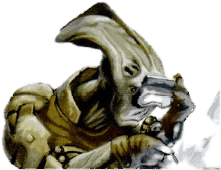
\includegraphics[width=\linewidth]{_img/dos-au-muur/vyna-anen.png}
\textbf{Race:} Sluissi

\subsubsection{Background}

Vyna Anen est l’un des agents de liaison entre Industrial Automaton et l’Empire. Officiellement employé par IA comme secrétaire au service des "Projets Spéciaux". 

Vyna est un homme pragmatique qui fait ce que l’Empire lui demande sans poser de questions, sans scrupules ni états d’âme. C’est un fin négociateur entièrement voué à l’Empire.

\subsubsection{Traits}

\begin{itemtable}[ c c c c c ]
    \textbf{Agi} & \textbf{Int} & \textbf{\^Ame} & \textbf{For} & \textbf{Vig} \\
    d6           & d10          & d6             & d4           & d6
\end{itemtable}
\begin{itemtable}[ l X ]
    \textbf{Allure}      & 6 \\
    \textbf{Compétences} & Intimidation d6, Persuasion d12, Réseaux d6
\end{itemtable}

\subsubsection{Défense}
\begin{itemtable}[ c c ]
    \textbf{Parade}     & \textbf{Résistance} \\
    2                   & 5 
\end{itemtable} 

\clearpage
\subsection{R4-3D*} \label{sec:r4-3d}

\clearpage
\subsection{Tinon Dystra} \label{sec:tinon-dystra}
\begin{figure}[h!]
    \centering
    
\includegraphics[height=250pt]{_img/dos-au-muur/tinon-dystra.png}
\end{figure}

\subsubsection{Background}
Ce personnage est mort quand débute le scénario mais il garde son importance car il est le lien entre les joueurs et l'alliance Rebelle.

Tinon est un membre de l'alliance rebelle envoyé en mission d'infiltration sur un vaisson de Industrial Automaton (Le \nameref{sec:pelican}) afin de découvrir ce qu'il s'y trame. Mais sa mission à mal tourné et il n'a plus donné aucune nouvelle. 

En fait il s'est infiltré à bord du Pelican alors que la maladie des \nameref{sec:rakghoul} était en train de s'y répandre. A bord du Pelican il s'est fait infecté et s'est transformé en Rakghoul lui-même. Son vaisseau, le \nameref{sec:nimbus} est resté à quai sur le Pelican.

Tinon avait une relation avec \nameref{sec:lindi-dangon}.

\newpage
\subsection{Lindi Dangon} \label{sec:lindi-dangon}
\begin{figure}[h!]
    \centering
    
\includegraphics[height=250pt]{_img/dos-au-muur/lindi-dangon.png}
\end{figure}
\subsubsection{Background}
Lindi Dangon commande l'une des cellule de résistance dans la zone de Taris. C'est elle qui a ordonné la mission durant laquelle \nameref{sec:tinon-dystra} à disparut. Elle se sent d'autant plus coupable que Tinon était son amant et depuis sa disparition elle n'a de sesse de la retrouver. Elle garde espoir tant qu'elle n'a pas de preuve de sa mort.

\subsubsection{Traits}

\begin{itemtable}[ c c c c c ]
    \textbf{Agi} & \textbf{Int} & \textbf{\^Ame} & \textbf{For} & \textbf{Vig} \\
    d6           & d10          & d8             & d4           & d4           
\end{itemtable}
\begin{itemtable}[ l X ]
    \textbf{Allure}      & 6 \\
    \textbf{Compétences} & Intimidation d8, Persuasion d8, Réseaux d10, Tir d10, Combat d4 \\
    \textdb{Atouts}      & Commandement
\end{itemtable}

\subsubsection{Défense}
\begin{itemtable}[ c c ]
    \textbf{Parade}     & \textbf{Résistance} \\
    5                   & 3 
\end{itemtable}

\newpage
\subsection{Garan Keggle}  \label{sec:garan-keggle}
\begin{figure}[h!]
    \centering
    
\includegraphics[height=200pt]{_img/dos-au-muur/garan-keggle.png}
\end{figure}
\vspace{-1\baselineskip}
\subsubsection{Background}
Officier supérieur dans l'armée de l'empire, Garan Keggle dirige les recherches d'artéfacts Sith pour le compte de l'empereur et son second Dark Vador. Suite à des informations sur le Talisman de Muur, il a dépéché un vaisseau de l'Insdustrial Automaton pour récupérer l'artéfact sur Taris sous couvert de projet scientifique.

Son contact chez IA est \nameref{sec:vyna-anen}, de manière générale Garan n'a que très peu de contact avec ses sous-traitant pour éviter que les ennuis remontent jsuqu'à l'empire. 

Garan est un home déterminé et sans pitié, initié au coté obscur de la Force, il attend la première occasion pour se débarrasser de ses rivaux et pouvoir prétendre au plus vite à la place d'apprenti et plus tard de seigneur Sith.

\subsubsection{Traits}
\begin{itemtable}[ c c c c c ]
    \textbf{Agi} & \textbf{Int} & \textbf{\^Ame} & \textbf{For} & \textbf{Vig} \\
    d6           & d10          & d10            & d6           & d8           
\end{itemtable}
\begin{itemtable}[ l X ]
    \textbf{Allure}      & 6 \\
    \textbf{Compétences} & Intimidation d10, Tir d10, Combat d8, Maitrise Force d8, Perception d6 \\
    \textdb{Atouts}      & Commandement, Grande aura de commandement
\end{itemtable}

\subsubsection{Défense}
\begin{itemtable}[ c c ]
    \textbf{Parade}     & \textbf{Résistance} \\
    6                   & 6 
\end{itemtable}

\newpage
\subsection{Gil Harend}  \label{sec:gil-harend}
\begin{figure}[h!]
    \centering
    
\includegraphics[height=200pt]{_img/dos-au-muur/gil-harend.png}
\end{figure}
\subsubsection{Background}
Double background selon la voie choisie.

Gil Harend est un père qui essai tant bien que mal d'élever sa fille de 16 ans, Abygaelle, dans les bas fonds de Taris. Depuis la disparition se sa femme Karie, la vie est très difficile. De plus les contrebandiers font régulièrement des razzia dans leur village pour kidnapper les jeunes filles et les revendre comme esclaves. Il y a deux jours, c'est Abygaelle qui a été enlevée. Gil fera tout pour la retrouver.\\

Gil Harend est un contrebandier qui opère dans les bas fonds de Taris. Avec ses 3 accolytes Gil fait des petits boulots plus ou moins légaux mais ce qui rapporte le plus c'est la revente de jeunes esclaves. Il y a 2 jours, lui est son équipe on kidnappés une jeune fille de 16 ans dans un village des bas fonds.

\subsubsection{Traits}
\begin{itemtable}[ c c c c c ]
    \textbf{Agi} & \textbf{Int} & \textbf{\^Ame} & \textbf{For} & \textbf{Vig} \\
    d4           & d8           & d4             & d8           & d8           
\end{itemtable}
\begin{itemtable}[ l X ]
    \textbf{Allure}      & 6 \\
    \textbf{Compétences} & Tir d6, Combat d4, Persuasion d6
\end{itemtable}

\subsubsection{Défense}
\begin{itemtable}[ c c ]
    \textbf{Parade}     & \textbf{Résistance} \\
    4                   & 6 
\end{itemtable}

\newpage
\subsection{Pulsipher} \label{sec:pulsipher}
\begin{figure}[h!]
    \centering
    
\includegraphics[height=200pt]{_img/dos-au-muur/pulsipher.png}
\end{figure}

\subsubsection{Background}
Pulsipher est un Mandalorien qui vécut plus de 3000 ans avant l'avènement de l'empire. Scientifique Néo-Croisé, il s'intéressait à la Force et tout ce qui s'y rattache. Il était persuadé que le secret de la Force lui permettrait de mettre fin à la guerre. 

C'est lui qui découvrit dans les bas-fonds de Taris et qui le ramena sur Jebble.

\subsubsection{Traits}
\begin{itemtable}[ c c c c c ]
    \textbf{Agi} & \textbf{Int} & \textbf{\^Ame} & \textbf{For} & \textbf{Vig} \\
    d4           & d12          & d4             & d8           & d6           
\end{itemtable}
\begin{itemtable}[ l X ]
    \textbf{Allure}      & 6 \\
    \textbf{Compétences} & Tir d8, Combat d8, Persuasion d6, Connaissance d12
\end{itemtable}

\subsubsection{Défense}
\begin{itemtable}[ c c ]
    \textbf{Parade}     & \textbf{Résistance} \\
    6                   & 8 
\end{itemtable}

\newpage
\subsection{Lucy} \label{sec:lucy-pher}
\begin{figure}[h!]
    \centering
    
\includegraphics[height=200pt]{_img/dos-au-muur/lucy.png}
\end{figure}

\subsubsection{Background}
Lucy est une IA particulièrement avancée (même pour la période du JdR). Mise au point par Pulsipher lui-même a partir d’un modèle de base, elle est la gardienne du Laboratoire et de tout se qu’il renferme. \'A l’époque où le labo était en activité, Lucy prenait en charge la plupart des caculs à effectuer sur l’ensemble des recherches. Elle était même capable d’anticiper certains résultats et d’ajuster les expériences de manière proactive.

Elle possède un plein accès au laboratoire, et par un réseau de caméra elle peut tout y voir.

\subsubsection{Traits}
\begin{itemtable}[ c c c c c ]
    \textbf{Agi} & \textbf{Int} & \textbf{\^Ame} & \textbf{For} & \textbf{Vig} \\
    d0           & d12+4        & d0             & d0           & d8           
\end{itemtable}
\begin{itemtable}[ l X ]
    \textbf{Allure}      & 0 \\
    \textbf{Compétences} & Tir d10, Combat d0, Persuasion d10, Connaissance d12
\end{itemtable}

\subsubsection{Défense}
\begin{itemtable}[ c c ]
    \textbf{Parade}     & \textbf{Résistance} \\
    0                   & 6 
\end{itemtable}

\newpage
\subsection{Céleste Morne*} \label{sec:celeste-morne}
\begin{figure}[h!]
    \centering
    
\includegraphics[height=200pt]{_img/dos-au-muur/celeste-morne.png}
\end{figure}

\subsubsection{Background}
Issue d’une famille de Jedi établie à Ossus, elle perdie tout ce qu’elle avait quand les Siths dévastèrent la planète durant la grande guerre des Siths. Sous la tutelle de Krynda Draay elle fut formée aux arts Jedi et, après une formation d’Ombre Jedi, elle fut recruté par le Covenant.

C’est en tant qu’Ombre du Covenant qu’elle partie en mission pour retrouver le Talisman de Muur et qu’elle croisa la route de \nameref{sec:pulsipher}. Lors de sa tentative pour sauver ce dernier et pour récupérer l’artéfact, celui-ci, attiré par les pouvoir de Céleste pris possession de son corps. Céleste parveint à le maitriser juste assez longtemps pour que Zayne Carrick, son apprenti l’enferme dans l’\nameref{sec:oubliette-de-dreypa}.

\subsubsection{Traits}
\begin{itemtable}[ c c c c c ]
    \textbf{Agi} & \textbf{Int} & \textbf{\^Ame} & \textbf{For} & \textbf{Vig} \\
    d10          & d8           & d10            & d6           & d8           
\end{itemtable}
\begin{itemtable}[ l X ]
    \textbf{Allure}      & 0 \\
    \textbf{Compétences} & Tir d6, Combat d12, Persuasion d10, Maitrise de la force d12
\end{itemtable}

\subsubsection{Défense}
\begin{itemtable}[ c c ]
    \textbf{Parade}     & \textbf{Résistance} \\
    8                   & 6 
\end{itemtable}

\newpage
\subsection{Fane Peturri} \label{sec:fane-peturri}
\begin{figure}[h!]
    \centering
    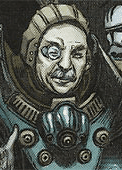
\includegraphics[height=200pt]{_img/dos-au-muur/fane-peturri.png}
\end{figure}

\subsubsection{Background}
Fane Peturri était un historien qui vécut durant les derniers décennies de la République et au tout début de l'Empire. Il semble qu'il était également un vieil ami de Palpatine et un des rares à savoir que celui-ci était un Seigneur Sith, ce qui fit qu'il eut des liens étroits avec l'Empire dès sa proclamation.

\subsubsection{Traits}
\begin{itemtable}[ c c c c c ]
    \textbf{Agi} & \textbf{Int} & \textbf{\^Ame} & \textbf{For} & \textbf{Vig} \\
    d6           & d10          & d4             & d6           & d8           
\end{itemtable}
\begin{itemtable}[ l X ]
    \textbf{Allure}      & 6 \\
    \textbf{Compétences} & Tir d4, Réseau d10, Connaissance (Empire) d10, Connaissance (Sith) d10
\end{itemtable}

\subsubsection{Défense}
\begin{itemtable}[ c c ]
    \textbf{Parade}     & \textbf{Résistance} \\
    4                   & 6 
\end{itemtable}

\newpage
\subsection{Schurk-Heren} \label{sec:schurk-heren}

\newpage
\subsection{Dass Jennir} \label{sec:dass-jennir}